% Options for packages loaded elsewhere
\PassOptionsToPackage{unicode}{hyperref}
\PassOptionsToPackage{hyphens}{url}
%
\documentclass[
  a4paperpaper,
]{report}
\usepackage{lmodern}
\usepackage{amssymb,amsmath}
\usepackage{ifxetex,ifluatex}
\ifnum 0\ifxetex 1\fi\ifluatex 1\fi=0 % if pdftex
  \usepackage[T2]{fontenc}
  \usepackage[utf8]{inputenc}
  \usepackage{textcomp} % provide euro and other symbols
\else % if luatex or xetex
  \usepackage{unicode-math}
  \defaultfontfeatures{Scale=MatchLowercase}
  \defaultfontfeatures[\rmfamily]{Ligatures=TeX,Scale=1}
  \setmainfont[]{Source Sans Pro}
\fi
% Use upquote if available, for straight quotes in verbatim environments
\IfFileExists{upquote.sty}{\usepackage{upquote}}{}
\IfFileExists{microtype.sty}{% use microtype if available
  \usepackage[]{microtype}
  \UseMicrotypeSet[protrusion]{basicmath} % disable protrusion for tt fonts
}{}
\makeatletter
\@ifundefined{KOMAClassName}{% if non-KOMA class
  \IfFileExists{parskip.sty}{%
    \usepackage{parskip}
  }{% else
    \setlength{\parindent}{0pt}
    \setlength{\parskip}{6pt plus 2pt minus 1pt}}
}{% if KOMA class
  \KOMAoptions{parskip=half}}
\makeatother
\usepackage{xcolor}
\IfFileExists{xurl.sty}{\usepackage{xurl}}{} % add URL line breaks if available
\IfFileExists{bookmark.sty}{\usepackage{bookmark}}{\usepackage{hyperref}}
\hypersetup{
  pdftitle={Analysis of the Russian Language},
  pdfauthor={Zubair Abid (20171076)},
  hidelinks,
  pdfcreator={LaTeX via pandoc}}
\urlstyle{same} % disable monospaced font for URLs
\usepackage{longtable,booktabs}
% Correct order of tables after \paragraph or \subparagraph
\usepackage{etoolbox}
\makeatletter
\patchcmd\longtable{\par}{\if@noskipsec\mbox{}\fi\par}{}{}
\makeatother
% Allow footnotes in longtable head/foot
\IfFileExists{footnotehyper.sty}{\usepackage{footnotehyper}}{\usepackage{footnote}}
\makesavenoteenv{longtable}
\usepackage{graphicx,grffile}
\makeatletter
\def\maxwidth{\ifdim\Gin@nat@width>\linewidth\linewidth\else\Gin@nat@width\fi}
\def\maxheight{\ifdim\Gin@nat@height>\textheight\textheight\else\Gin@nat@height\fi}
\makeatother
% Scale images if necessary, so that they will not overflow the page
% margins by default, and it is still possible to overwrite the defaults
% using explicit options in \includegraphics[width, height, ...]{}
\setkeys{Gin}{width=\maxwidth,height=\maxheight,keepaspectratio}
% Set default figure placement to htbp
\makeatletter
\def\fps@figure{htbp}
\makeatother
\setlength{\emergencystretch}{3em} % prevent overfull lines
\providecommand{\tightlist}{%
  \setlength{\itemsep}{0pt}\setlength{\parskip}{0pt}}
\setcounter{secnumdepth}{-\maxdimen} % remove section numbering

\title{Analysis of the Russian Language}
\author{Zubair Abid (20171076)}
\date{}

\begin{document}
\maketitle

{
\setcounter{tocdepth}{2}
\tableofcontents
}
\hypertarget{introduction-and-language-family}{%
\chapter{Introduction and Language
Family}\label{introduction-and-language-family}}

Russian is an \textbf{Indo-European} language - one of the four living
\texttt{East-Slavic} languages, which is a subset of the
\texttt{Common\ Slavic} languages.

With over 160 million native speakers, it is the 8th most
natively-spoken language in the world, and also the most geographically
widespread language in Eurasia. Native speakers of Russian include not
only the Russian people, but also people from several countries
belonging to erstwhile USSR. Among these, it is an official language in
the Russian Federation, Belarus, Kazakhstan and Kyrgyzstan.

\begin{figure}
\centering
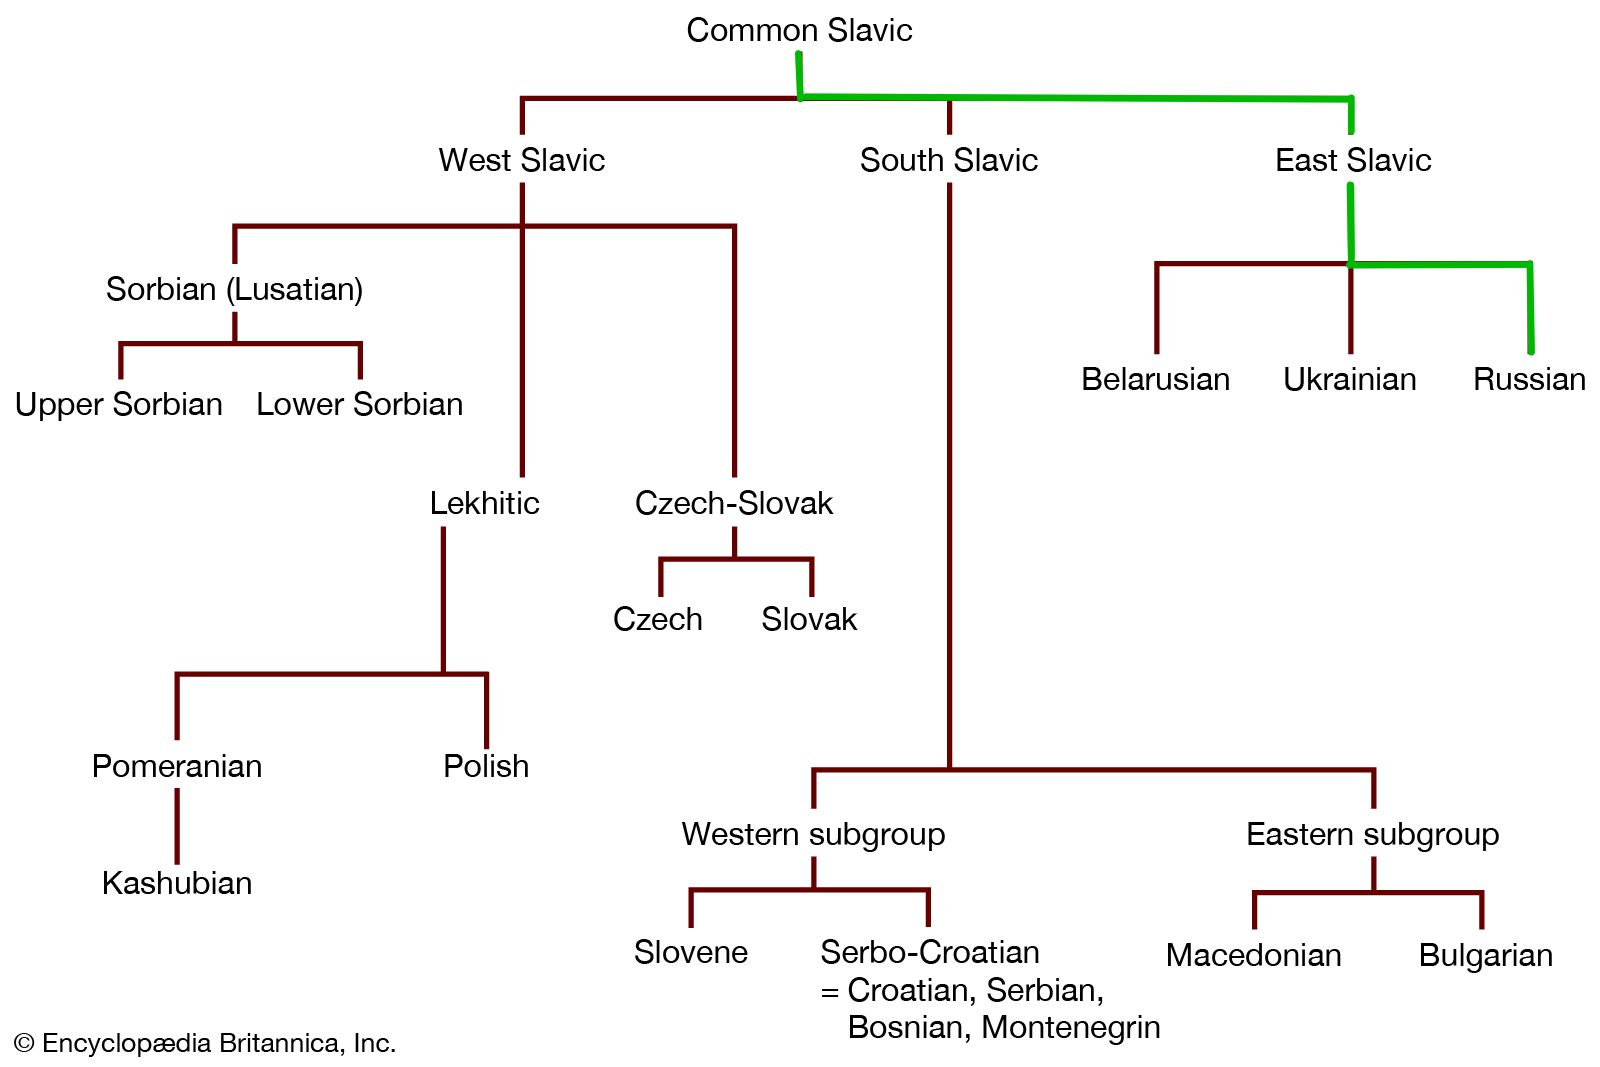
\includegraphics{./russtree_russ.jpg}
\caption{Family tree of the Slavic Languages}
\end{figure}

\begin{figure}
\centering
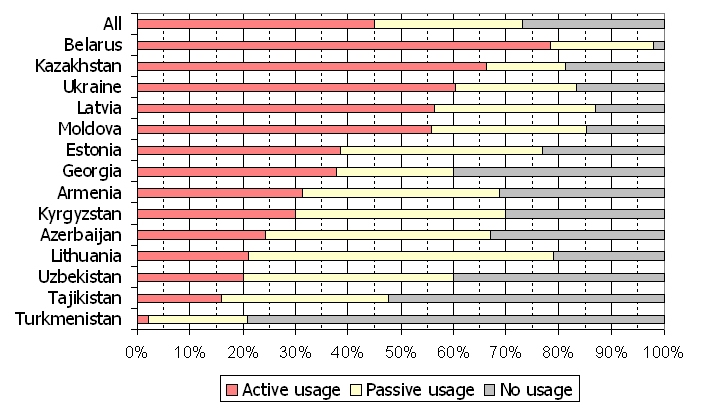
\includegraphics{./russian_usage.PNG}
\caption{Competence of Russian in countries of the former Sovier Union}
\end{figure}

\begin{figure}
\centering
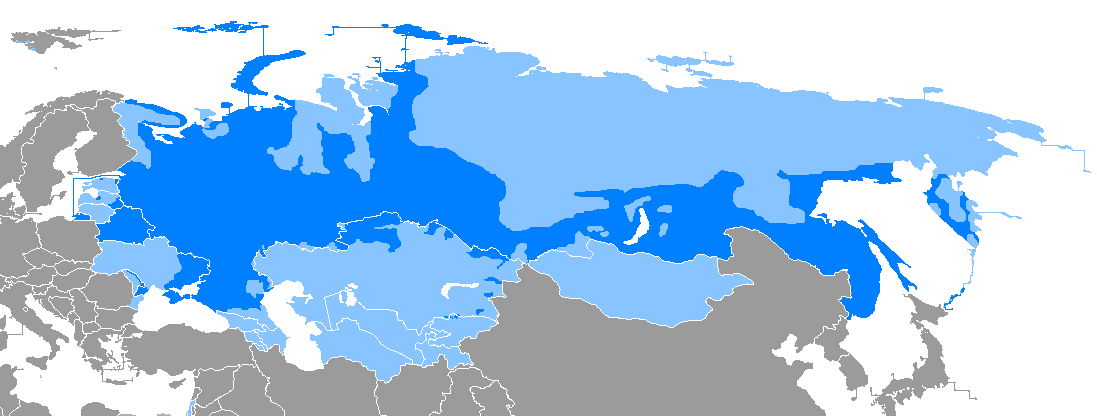
\includegraphics{./Idioma_ruso.PNG}
\caption{Areas where Russian is the majority language (medium blue) or a
minority language (light blue)}
\end{figure}

\hypertarget{important-features-of-the-language}{%
\section{Important Features of the
Language}\label{important-features-of-the-language}}

Amongst other important features of the language, some of the more
prominent ones are:

\begin{itemize}
\tightlist
\item
  Widespread palatalization of consonants. This is also present in other
  Slavic Languages.
\item
  There is extensive nominal morphology, a holdover from the complexity
  of old Indo-European languages. It is most notable in its declension
  system
\item
  The verb system is simpler, with only two basic verbs.
\end{itemize}

\hypertarget{dialects-of-russian}{%
\section{Dialects of Russian}\label{dialects-of-russian}}

There are three notable dialects of Russian that can be distinguished by
their pronunciation:

\begin{itemize}
\tightlist
\item
  \textbf{The Nothern Dialect}, spoken from St.~Petersburg eastwards
  across Siberia
\item
  \textbf{The Souther Dialect}, spoken in most of Central and Southern
  Russia
\item
  \textbf{The Central Dialect}, in between the two above.
\end{itemize}

\hypertarget{orthography}{%
\chapter{Orthography}\label{orthography}}

Russian uses the \textbf{Cyrillic alphabet} (`Russian' is written
русский - {[}ˈruskʲɪj{]} in Cyrillic). It is derived from a script
created between 800-900 AD, based on the Greek uncial script.

\begin{itemize}
\tightlist
\item
  There are 32 letters and an \emph{additional sign for palatalization}
  \footnote{This is sometimes reported as 33 letters. I have kept the
    `additional sign for palatalization'}

  \begin{itemize}
  \tightlist
  \item
    Ь indicates palatalization of the previous consonant.
  \item
    Ъ is silent; it prevents palatalization of the preceding consonant.
  \end{itemize}
\item
  Stress is not normally indicated orthographically. An optional acute
  accent is used to mark it when distinguishing between homographic
  words.
\end{itemize}

\begin{figure}
\centering
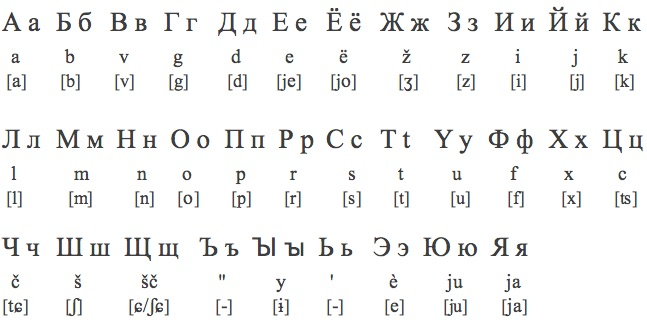
\includegraphics{./script.jpg}
\caption{The Cyrillic Script, transliteration, and IPA transcription}
\end{figure}

\hypertarget{phonology-and-phonetics}{%
\chapter{Phonology and Phonetics}\label{phonology-and-phonetics}}

\hypertarget{vowels}{%
\section{Vowels}\label{vowels}}

Russian has a surprisingly low number of vowel sounds, at 5 - or 6, if
you subscribe to the St.~Petersburg Phonological School. This confusion
arises from the phonemic status of the i/ɨ alternation:

\begin{itemize}
\tightlist
\item
  ɨ occurs only after non-palatalized consonants
\item
  i only after palatalized ones and word-initially
\end{itemize}

They could be considered either complementary sounds or separate
phonemes.

The reduced i and u vowels of the ancestral Slavic language were lost in
Russian.

\begin{longtable}[]{@{}llll@{}}
\caption{Vowel Chart in Russian}\tabularnewline
\toprule
& \textbf{Front} & \textbf{Central} & \textbf{Back}\tabularnewline
\midrule
\endfirsthead
\toprule
& \textbf{Front} & \textbf{Central} & \textbf{Back}\tabularnewline
\midrule
\endhead
\textbf{Mid} & i & (ɨ) & u\tabularnewline
\textbf{Mid} & e & & o\tabularnewline
\textbf{Low} & & a &\tabularnewline
\bottomrule
\end{longtable}

\begin{figure}
\centering
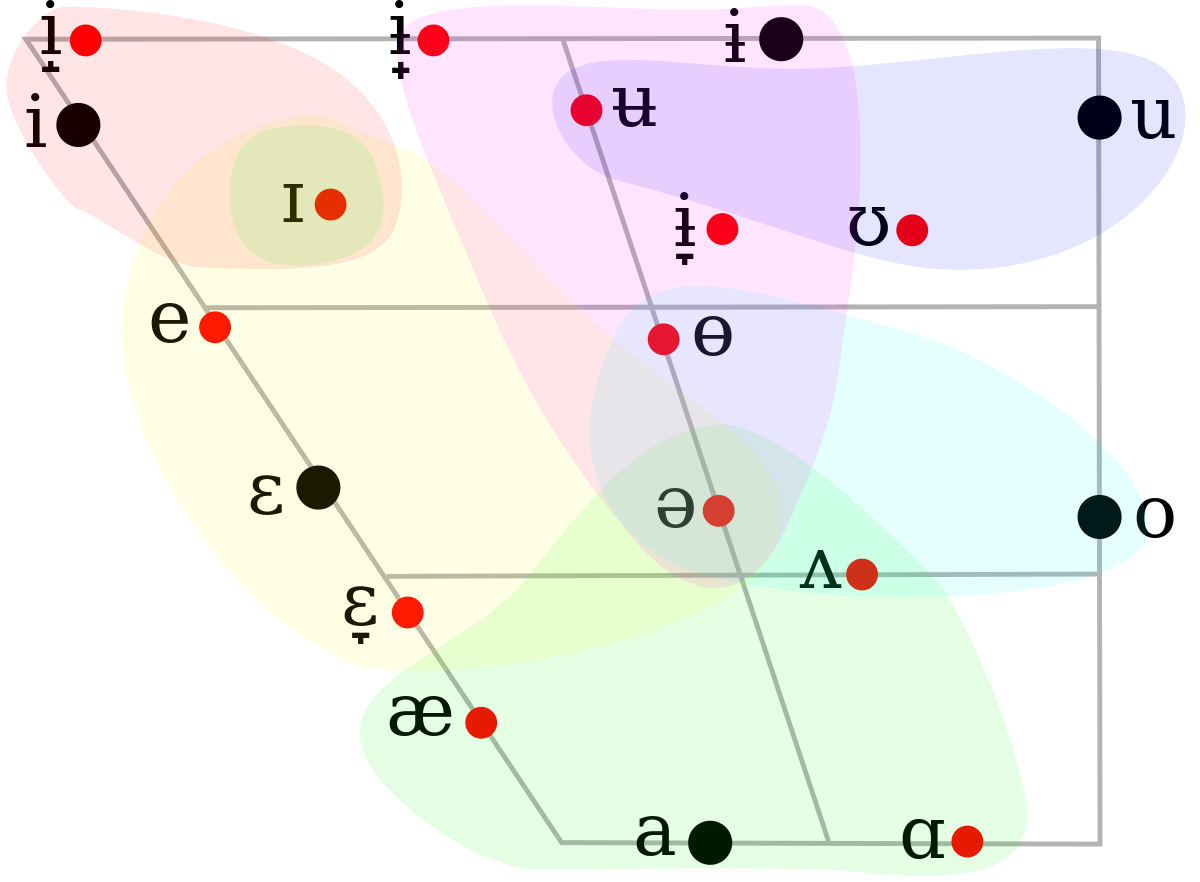
\includegraphics[width=0.6\textwidth,height=\textheight]{./vowels.png}
\caption{Russian Vowel Chart by Jones and Trofimov}
\end{figure}

\hypertarget{consonants}{%
\section{Consonants}\label{consonants}}

Russian has 36 consonants. Consonant palatalization is widespread, as
mentioned earlier: only three consonants lack palatalized counterparts:

\begin{itemize}
\tightlist
\item
  \textbf{{[}ts{]}}, \textbf{{[}ʃ{]}}, \textbf{{[}ʒ{]}} lack palatalized
  counterparts.
\item
  \textbf{{[}tɕ{]}}, \textbf{{[}ɕ{]}}, \textbf{{[}j{]}}, are always
  palatalized, lacking counterparts.
\end{itemize}

Palatalization is represented by an accent mark over the letter.

\begin{longtable}[]{@{}lllllll@{}}
\caption{Consonant chart}\tabularnewline
\toprule
& & \textbf{Labial} & \textbf{Dental} & \textbf{Alveopalatal} &
\textbf{Palatal} & \textbf{Velar}\tabularnewline
\midrule
\endfirsthead
\toprule
& & \textbf{Labial} & \textbf{Dental} & \textbf{Alveopalatal} &
\textbf{Palatal} & \textbf{Velar}\tabularnewline
\midrule
\endhead
\textbf{Stop} & Voiceless & p ṕ & t t' & & & k ḱ\tabularnewline
& Voiced & b b' & d d' & & & g ǵ\tabularnewline
\textbf{Affricate} & \emph{Voiceless} & & ts & & tɕ &\tabularnewline
\textbf{Fricative} & \emph{Voiceless} & f f' & s ś & ʃ & ɕ & x
x'\tabularnewline
& \emph{Voiced} & v v' & z ź & ʒ & &\tabularnewline
\textbf{Nasal} & & m ḿ & n ń & & &\tabularnewline
\textbf{Trill} & & & l ĺ & & &\tabularnewline
\textbf{Approximant} & & & r ŕ & & j &\tabularnewline
\bottomrule
\end{longtable}

\hypertarget{stress}{%
\section{Stress}\label{stress}}

Stress can fall on any syllable and it may serve to differentiate
lexical or morphological forms. For instance, muká (`flour') versus múka
(`torment'), rukí (genitive singular) versus rúki (nominative plural).

Stress is not normally indicated orthographically. An optional acute
accent is used to mark it when distinguishing between homographic words.

\hypertarget{syllable-structure}{%
\section{Syllable Structure}\label{syllable-structure}}

Syllable structure can be complicated, wih inital and final consonant
clusters of upto 4 consecutive sounds:
\textbf{(C)(C)(C)(C)V(C)(C)(C)(C)} is the maximal structure of the
russian syllable.

These clusters are not very common. Examples: - взгляд ({[}vzglʲat{]},
`glance') - государств ({[}gəsʊˈdarstf{]}, `of the states')

However, syllables cannot span multiple morphemes.

\hypertarget{morphology}{%
\chapter{Morphology}\label{morphology}}

Russian Morphology is \textbf{highly fusional}

\hypertarget{nouns}{%
\section{Nouns}\label{nouns}}

Russian nominal morphology has retained part of the complexity of Old
Church Slavonic.

However, it has lost:

\begin{itemize}
\tightlist
\item
  The vocative case
\item
  The number of declension types has been reduced
\item
  The dual number has disappeared
\end{itemize}

Definite and Indefinite Articles do not exist in the language.

\begin{longtable}[]{@{}ll@{}}
\caption{General characteristics covered under Nominal
Morphology}\tabularnewline
\toprule
\begin{minipage}[b]{0.16\columnwidth}\raggedright
\textbf{Property}\strut
\end{minipage} & \begin{minipage}[b]{0.78\columnwidth}\raggedright
\textbf{Values}\strut
\end{minipage}\tabularnewline
\midrule
\endfirsthead
\toprule
\begin{minipage}[b]{0.16\columnwidth}\raggedright
\textbf{Property}\strut
\end{minipage} & \begin{minipage}[b]{0.78\columnwidth}\raggedright
\textbf{Values}\strut
\end{minipage}\tabularnewline
\midrule
\endhead
\begin{minipage}[t]{0.16\columnwidth}\raggedright
\textbf{Gender}\strut
\end{minipage} & \begin{minipage}[t]{0.78\columnwidth}\raggedright
masculine, neuter, feminine\strut
\end{minipage}\tabularnewline
\begin{minipage}[t]{0.16\columnwidth}\raggedright
\textbf{Number}\strut
\end{minipage} & \begin{minipage}[t]{0.78\columnwidth}\raggedright
singular, plural\strut
\end{minipage}\tabularnewline
\begin{minipage}[t]{0.16\columnwidth}\raggedright
\textbf{Case}\strut
\end{minipage} & \begin{minipage}[t]{0.78\columnwidth}\raggedright
nominative, accusative, genitive, dative, instrumental,
locative/prepositional\strut
\end{minipage}\tabularnewline
\begin{minipage}[t]{0.16\columnwidth}\raggedright
\textbf{Adjectives}\strut
\end{minipage} & \begin{minipage}[t]{0.78\columnwidth}\raggedright
masculine singular, neuter singular, feminine singular, plural\strut
\end{minipage}\tabularnewline
\begin{minipage}[t]{0.16\columnwidth}\raggedright
\textbf{Pronouns}\strut
\end{minipage} & \begin{minipage}[t]{0.78\columnwidth}\raggedright
personal, possessive, demonstrative, interrogative, relative\strut
\end{minipage}\tabularnewline
\bottomrule
\end{longtable}

\hypertarget{nouns-and-case}{%
\section{Nouns and Case}\label{nouns-and-case}}

Russian declensions involve 6 cases, although linguistics textbooks have
identified up to 10. Most of the extras, incomplete, have fallen out of
use over time. All 6 cases - nominative, genitive, dative, accusative,
instrumental, and prepositional - are in two numbers, and obey
absolutely the grammatical genders of masculine, feminine, and neuter.

Russian noun cases may supplant the use of prepositions entirely.
Moreover, every preposition is exclusively used with a particular case
(or cases).

Some examples of use are:

\begin{longtable}[]{@{}ll@{}}
\caption{Russian case usage}\tabularnewline
\toprule
\begin{minipage}[b]{0.13\columnwidth}\raggedright
\textbf{Case}\strut
\end{minipage} & \begin{minipage}[b]{0.81\columnwidth}\raggedright
\textbf{Use}\strut
\end{minipage}\tabularnewline
\midrule
\endfirsthead
\toprule
\begin{minipage}[b]{0.13\columnwidth}\raggedright
\textbf{Case}\strut
\end{minipage} & \begin{minipage}[b]{0.81\columnwidth}\raggedright
\textbf{Use}\strut
\end{minipage}\tabularnewline
\midrule
\endhead
\begin{minipage}[t]{0.13\columnwidth}\raggedright
nominative\strut
\end{minipage} & \begin{minipage}[t]{0.81\columnwidth}\raggedright
main subject; default outside sentences; prepositions\strut
\end{minipage}\tabularnewline
\begin{minipage}[t]{0.13\columnwidth}\raggedright
accusative\strut
\end{minipage} & \begin{minipage}[t]{0.81\columnwidth}\raggedright
direct object; time expressions; prepositions indicating motion\strut
\end{minipage}\tabularnewline
\begin{minipage}[t]{0.13\columnwidth}\raggedright
genitive\strut
\end{minipage} & \begin{minipage}[t]{0.81\columnwidth}\raggedright
possession; numerals; verbs; adjectives; other time expressions\strut
\end{minipage}\tabularnewline
\begin{minipage}[t]{0.13\columnwidth}\raggedright
dative\strut
\end{minipage} & \begin{minipage}[t]{0.81\columnwidth}\raggedright
indirect object; some other time expressions; impersonal clauses, age
statements, auxillaries\strut
\end{minipage}\tabularnewline
\begin{minipage}[t]{0.13\columnwidth}\raggedright
instrumental\strut
\end{minipage} & \begin{minipage}[t]{0.81\columnwidth}\raggedright
durational time expressions; secondary direct objects\strut
\end{minipage}\tabularnewline
\begin{minipage}[t]{0.13\columnwidth}\raggedright
prepositional\strut
\end{minipage} & \begin{minipage}[t]{0.81\columnwidth}\raggedright
prepositions of a place\strut
\end{minipage}\tabularnewline
\bottomrule
\end{longtable}

Russian has four major types of noun declension: a-stem, masculine
o-stem, neuter o-stem and i-stem.

\begin{itemize}
\tightlist
\item
  Most a-stem nouns are feminine (but those that refer to a male are
  masculine).
\item
  Almost all i-stems are feminine.
\item
  O-stem nouns are masculine or neuter.
\end{itemize}

\begin{figure}
\centering
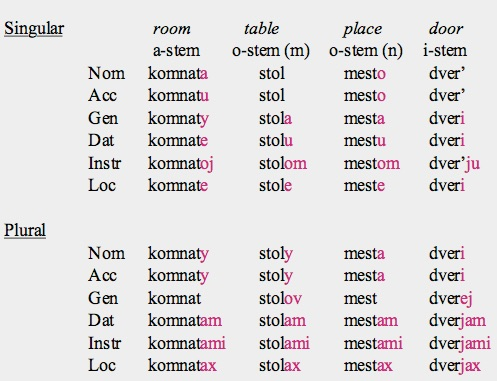
\includegraphics{./casedec.jpg}
\caption{Nouns and Case in Russian}
\end{figure}

\hypertarget{nouns-and-adjectives}{%
\section{Nouns and Adjectives}\label{nouns-and-adjectives}}

Nouns and adjectives in Russian are rather straightforward:

\begin{itemize}
\tightlist
\item
  Plural forms do not distinguish gender
\item
  Neuter and Masculine adjectives differ in nominative and accusative
\item
  Feminine sing. adjectives: one form for genitive, dative,
  instrumental, locative
\end{itemize}

\begin{figure}
\centering
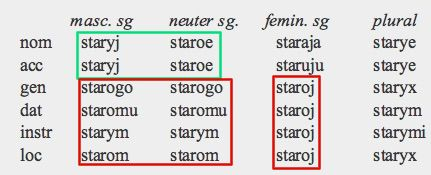
\includegraphics{./adj.jpg}
\caption{Declension of \emph{staryj} (old)}
\end{figure}

\hypertarget{nouns-and-pronouns}{%
\section{Nouns and Pronouns}\label{nouns-and-pronouns}}

Pronouns in Russian can be personal, possessive, demonstrative,
interrogative, or relative.

\hypertarget{personal-pronouns}{%
\subsection{Personal Pronouns}\label{personal-pronouns}}

\begin{itemize}
\tightlist
\item
  Declined in all 6 cases
\item
  Distinguish Gender in \textbf{3rd Person Singular}
\item
  2nd plural form may be used as a polite singular
\end{itemize}

\begin{figure}
\centering
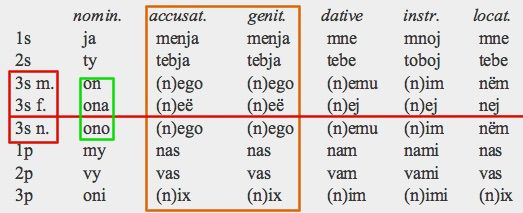
\includegraphics[width=0.8\textwidth,height=\textheight]{./perspron.jpg}
\caption{Personal pronouns in Russian}
\end{figure}

\hypertarget{possessive-pronounsadjectives}{%
\subsection{Possessive
Pronouns/Adjectives}\label{possessive-pronounsadjectives}}

\begin{itemize}
\tightlist
\item
  Declined in all cases
\item
  Distinguish gender in the singular, \textbf{Exception} of 3rd person
  forms
\end{itemize}

\begin{figure}
\centering
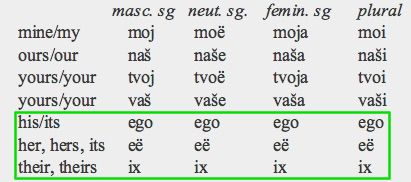
\includegraphics[width=0.8\textwidth,height=\textheight]{./pospron.jpg}
\caption{Possessive Pronouns}
\end{figure}

\hypertarget{demonstrative-adjectives}{%
\subsection{Demonstrative Adjectives}\label{demonstrative-adjectives}}

Neuter single forms are \emph{used as demonstrative pronouns}

\begin{figure}
\centering
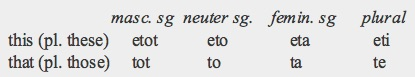
\includegraphics[width=0.6\textwidth,height=\textheight]{./demad.jpg}
\caption{Demonstrative Adjectives as Pronouns}
\end{figure}

\hypertarget{interrogative-pronouns}{%
\subsection{Interrogative Pronouns}\label{interrogative-pronouns}}

Mainly: kto (`who?') and čto (`what?')

Others: kotoryj (`what?/which?') and kakoj (`what kind of?').

All of the above can also function as relative pronouns.

\hypertarget{indefinite-pronouns}{%
\subsection{Indefinite pronouns}\label{indefinite-pronouns}}

Formed by adding \texttt{-to}/\texttt{-nibud} to interrogative pronouns.

\hypertarget{the-only-reflexive-pronoun}{%
\subsection{(The only) Reflexive
Pronoun}\label{the-only-reflexive-pronoun}}

\texttt{sebja} (`himself, herself')

\hypertarget{nouns-and-animacy}{%
\section{Nouns and Animacy}\label{nouns-and-animacy}}

\textbf{Animacy} is relevant in nominal and adjectival declensions.

The Accusative has two possible forms depending on animacy of the
referent

\begin{itemize}
\tightlist
\item
  For Animate referents (persons, animals), accusative is generally
  identical to genitive
\item
  For Inanimate referents, accusative is identical to nominative
\end{itemize}

\hypertarget{verbal}{%
\chapter{Verbal}\label{verbal}}

Compared to the nominal morphology, Russian verbal morphology is far
simpler. There are two basic non-compound tenses used, two aspects, two
moods, and two conjugation types.

\begin{itemize}
\tightlist
\item
  \textbf{Non-compound tenses:} past, non-past
\item
  \textbf{Aspects:} perfective, imperfective
\item
  \textbf{Moods:} indicative, imperative
\end{itemize}

The infinitive is the only non-finite form widely used.

\begin{longtable}[]{@{}ll@{}}
\caption{General characteristics covered under Verbal
Morphology}\tabularnewline
\toprule
\textbf{Property} & \textbf{Values}\tabularnewline
\midrule
\endfirsthead
\toprule
\textbf{Property} & \textbf{Values}\tabularnewline
\midrule
\endhead
\textbf{Person and Number} & 1s, 2s, 3s; 1p, 2p, 3p\tabularnewline
\textbf{Modality} & indicative, imperative\tabularnewline
\textbf{Tense} & past, non-past, imperfective future,
conditional\tabularnewline
\textbf{Aspect} & imperfective, perfective\tabularnewline
\textbf{Voice} & active, passive (infrequent)\tabularnewline
\bottomrule
\end{longtable}

\hypertarget{verbal-tense}{%
\section{Verbal, Tense}\label{verbal-tense}}

There are in total: \emph{past, non-past, imperfective future,
conditional}

\begin{itemize}
\tightlist
\item
  \emph{past, non-past}: are the only tenses formed without an auxiliary
\item
  \emph{non-past}: verbs agree with their subject in the \textbf{person,
  number}
\item
  \emph{past}: verbs agree with their subject in the \textbf{gender,
  number}, but not in person, as the tense derives from the participle
  form.
\item
  \emph{imperfective future}: It is formed by the
  auxiliary\texttt{budu}(`will be'), which is a future form of the verb
  `to be' plus the infinitive.
\item
  \emph{conditional}: It is formed by past tense + the invariable
  participle `by'
\end{itemize}

\begin{figure}
\centering
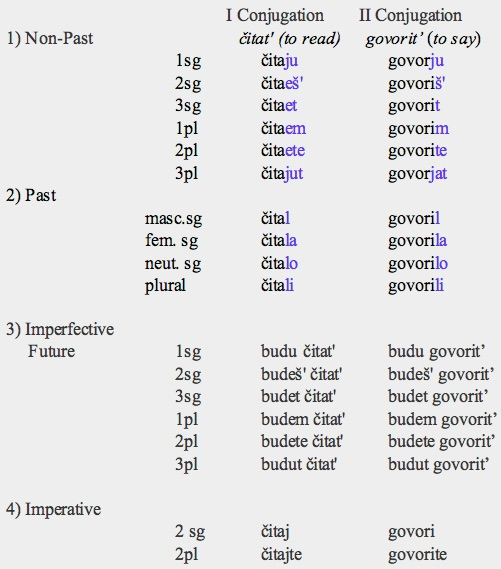
\includegraphics[width=0.6\textwidth,height=\textheight]{./tense.jpg}
\caption{Tenses}
\end{figure}

\hypertarget{verbal-aspect}{%
\section{Verbal, Aspect}\label{verbal-aspect}}

We examine two aspects: \emph{imperfective, perfective}

\begin{itemize}
\tightlist
\item
  \textbf{imperfective}: Denotes incomplete/ongoing action
\item
  \textbf{perfective}: Denotes completed action
\end{itemize}

The perfective is usually expressed by adding a prefix to the
imperfective form of the verb.

The prefix is unpredictable: It may change meaning of verb, or it may
not. In the example below, it does not change in 1 and 2, but it does in
the third.

\begin{enumerate}
\def\labelenumi{\arabic{enumi}.}
\tightlist
\item
  to read: čitat (imperfective), to read: pročitat (perfective)
\item
  to write: pisat (imperfective), to write: napisat (perfective)
\item
  to write: pisat (imperfective), to describe: opisat (perfective)
\end{enumerate}

\hypertarget{verbal-voice}{%
\section{Verbal, Voice}\label{verbal-voice}}

There is Active and Passive voice, but usage of Passive is infrequent.

\hypertarget{verbal-non-finite-forms}{%
\section{Verbal, Non-Finite forms}\label{verbal-non-finite-forms}}

The only common one is the \emph{infinitive}

Participles and Gerunds are only used in literary language. Of these,
there are 5:

\begin{itemize}
\tightlist
\item
  Present Active (`doing')
\item
  Present Passive (`being done')
\item
  Past Active Imperfective (`were doing')
\item
  Perfective (`having done')
\item
  Past Passive Perfective (`done')
\end{itemize}

There are also two adverbial participles (gerunds) that are
indeclinable.

\hypertarget{syntax}{%
\chapter{Syntax}\label{syntax}}

The word order of Russian is a very flexible Subject Verb Object (SVO).
The case system is enough to indicate function of words in sentences.

\hypertarget{whats-missing}{%
\section{What's missing}\label{whats-missing}}

There are no articles, and the Copula (the `to be' verb) is omitted in
the present tense

\hypertarget{positions-of-structures}{%
\section{Positions of structures}\label{positions-of-structures}}

Mostly,

Prepositions, rather than postpositions

Subordinate clauses follow main clauses

Adjectives precede nouns, and they agree in gender, number, case.

\hypertarget{agreement-of-finite-verbs}{%
\section{Agreement of finite verbs}\label{agreement-of-finite-verbs}}

Finite verbs agree with their subjects in:

\begin{itemize}
\tightlist
\item
  Person and number in the non past tense
\item
  Gender and number in the past tense
\end{itemize}

\hypertarget{semantics}{%
\chapter{Semantics}\label{semantics}}

\hypertarget{numbers}{%
\section{Numbers}\label{numbers}}

By and large, the russian counting system seems rather similar to
English, with words for digits and 11-19, and tens (desyat), hundreds
(sto), and thousands (tysyacha).

\begin{longtable}[]{@{}lllll@{}}
\caption{Numbers in Russian}\tabularnewline
\toprule
10,1-9 & 11-19 & 20,21,(30,90,10) & 100,147, (200,900,100) &
1000,2000\tabularnewline
\midrule
\endfirsthead
\toprule
10,1-9 & 11-19 & 20,21,(30,90,10) & 100,147, (200,900,100) &
1000,2000\tabularnewline
\midrule
\endhead
`desyat' & & & sto & tysyacha\tabularnewline
a'deen & o'dinnatdsat' & d'vadtsat' & sto sorok sem' &\tabularnewline
dva & dve'nadtsat & dvadsat' odeen & dvesti & dve
tysyachi\tabularnewline
tri & tri'nadsat' & t'ridtsat' & treesta &\tabularnewline
chetyre & che'tyrnadsat' & sorok & chetyresta &\tabularnewline
pyat' & pyat'nadtsat' & pyatdesyat & pyat'sot &\tabularnewline
shest & shet'nadtsat' & shestdesyat & shestsot &\tabularnewline
sem' & sem'nadtsat' & 'semdesyat & sem'sot &\tabularnewline
vosem' & vosem'nadtsat' & vosemdesyat & vosemsot &\tabularnewline
devyat' & devyat'nadtsat' & devyanosto & devyatsot &\tabularnewline
\bottomrule
\end{longtable}

\hypertarget{colours}{%
\section{Colours}\label{colours}}

Russian appears to be an exception to Berlin and Kay's suggestion that
languages should have a maximum of 11 basic colour terms.

Russian has 12. There's distinction between light and dark blue.

\emph{belyj} --\textgreater{} \emph{cernyj} --\textgreater{}
\emph{krasnyj} --\textgreater{} \emph{zelenyj} --\textgreater{}
\emph{zeltyj} --\textgreater{} \textbf{sinij} --\textgreater{}
\textbf{goluboj}--\textgreater{} \emph{koricnevyj} --\textgreater{}
\emph{fioletovyj} --\textgreater{} \emph{rozovyj} --\textgreater{}
\emph{oranzevyj} --\textgreater{} \emph{seryj}

white --\textgreater{} black --\textgreater{} red --\textgreater{} green
--\textgreater{} yellow --\textgreater{} \emph{dark blue}
--\textgreater{} \emph{light blue} --\textgreater{} brown
--\textgreater{} purple --\textgreater{} pink --\textgreater{} orange
--\textgreater{} grey

\hypertarget{kinship-terms}{%
\section{Kinship terms}\label{kinship-terms}}

Relationship terms exist for:

\begin{longtable}[]{@{}ll@{}}
\toprule
English Word & Russian Word\tabularnewline
\midrule
\endhead
family & семья́ (sem'ya)\tabularnewline
parents & роди́тели (roditeli)\tabularnewline
father & оте́ц (otec)\tabularnewline
mother & мать (mat')\tabularnewline
children & де́ти (deti)\tabularnewline
son & сын (syn)\tabularnewline
daughter & дочь (doč')\tabularnewline
husband & муж (muž)\tabularnewline
wife & жена́ (žena)\tabularnewline
brother & брат (brat)\tabularnewline
sister & сестра́ (sestra)\tabularnewline
uncle & дя́дя (djadja)\tabularnewline
aunt & тётя (tjotja)\tabularnewline
cousin & кузе́н (kuzen) - m\tabularnewline
& кузи́на (kuzina) - f\tabularnewline
& двою́родный брат (dvojurodmyj brat) - m\tabularnewline
& двою́родная сестра́ (dvojurodnaja sestra) - f\tabularnewline
second cousin & трою́родный брат (trojurodnyj brat) - m\tabularnewline
& трою́родная сестра́ (trojurodnaja sestra) - f\tabularnewline
nephew & племя́нник (plemjannik)\tabularnewline
niece & племя́нница (plemjannica)\tabularnewline
grandparents & де́душка и\tabularnewline
& ба́бушка (deduška i babuška)\tabularnewline
grandfather & дед (ded) де́душка (deduška)\tabularnewline
grandmother & ба́бка (babka)\tabularnewline
& ба́бушка (babuška)\tabularnewline
grandchildren & вну́ки (vnuki)\tabularnewline
grandson & внук (vnuk)\tabularnewline
granddaughter & вну́чка (vnučka)\tabularnewline
great uncle & двою́родный дед (dvojurodnyj ded)\tabularnewline
great aunt & двою́родная ба́бка (dvojurodnaja babka)\tabularnewline
grandnephew & внуча́тый племя́нник (vnučatyj plemjannik)\tabularnewline
grandniece & внуча́тая племя́нница (vnučataja plemjannica)\tabularnewline
great grandfather & пра́дед (praded) праде́душка
(pradeduška)\tabularnewline
great grandmother & праба́бка (prababka) праба́бушка
(prababuška)\tabularnewline
great grandson & пра́внук (pravnuk)\tabularnewline
great granddaughter & пра́внучка (pravnučka)\tabularnewline
father-in-law & свёкор (svjokor) husband's father\tabularnewline
& тесть (test') wife's father\tabularnewline
mother-in-law & свекро́вь (svekrov') husband's mother\tabularnewline
& тёща (tjošča) wife's mother\tabularnewline
brother-in-law & зять (zjat') sister's husband\tabularnewline
& шу́рин (šurin) wife's brother\tabularnewline
& де́верь (dever') husband's brother\tabularnewline
& своя́к (svojak) wife's sister's husband\tabularnewline
sister-in-law & неве́стка (nevestka) brother's wife\tabularnewline
& золо́вка (zolovka) husband's sister\tabularnewline
& своя́ченица (svojačenitsa) wife's sister\tabularnewline
son-in-law & зять (zjat')\tabularnewline
daughter-in-law & неве́стка (nevestka)\tabularnewline
& сноха́ (snoxa)\tabularnewline
stepfather & о́тчим (otčim)\tabularnewline
stepmother & ма́чеха (mačexa)\tabularnewline
stepson & па́сынок (pasynok)\tabularnewline
stepdaughter & па́дчерица (padčerica)\tabularnewline
\bottomrule
\end{longtable}

\begin{itemize}
\tightlist
\item
  Immediate blood relations
\item
  Great uncles/aunts
\item
  In-laws
\item
  Paternal/maternal distinction of grandparents/cousins
\item
  No Paternal/maternal distinction of uncles/aunts
\item
  Male/female distinction of cousins
\item
  Male/female distinction of second cousins
\item
  Step-family
\item
  Great grandparents/grandchildren
\end{itemize}

\end{document}
